\documentclass[titlepage]{article}
\usepackage[utf8]{inputenc}
\usepackage[T1]{fontenc}
\usepackage[colorlinks=false]{hyperref}
%\usepackage[a4paper, margin=3cm]{geometry}
\usepackage{graphicx}
\usepackage{listings} % to display code snippets
\usepackage{xcolor}  % Optional, for coloring code


\title{Software Engineering Project}
\author{Daniel \sc Carriba Nosrati}
\date{2025}

\renewcommand{\contentsname}{Sommaire}
\hyphenpenalty=10000  % Empêche la coupure des mots en fin de ligne
\exhyphenpenalty=10000  % Empêche aussi la coupure des mots avec des apostrophes


\begin{document}


\begin{titlepage}
    \centering
    \vspace*{\fill}
    {
\includegraphics[width=0.5\textwidth]{img/unice-logo.png} \par}
    \vfill
    {\Huge \bfseries Software Engineering\\Project \par}
    \vspace{1cm}
    {\Large Compression de données pour accélérer la transmission \par}
    \vfill
    {\Large Daniel \sc Carriba Nosrati \par}
    \vspace{0.5cm}
    {\large UE Software Engineering\\Semestre 1 Master 1 Informatique\\Université Côte d'Azur \par}
    \vspace{0.5cm}
    {\large 2025 \par}
    \vspace*{\fill} 
\end{titlepage}


\tableofcontents

\clearpage




\section{Introduction}

Ce projet, réalisé pour l'UE "Software Engineering" du Semestre 1 du Master 1 Informatique de l'Université Côte d'Azur, est un projet sur le thème de compression de données pour accélérer la transmission.
\par La transmission de tableaux d'entiers est un problème majeur de l'internet. Ce projet propose une réponse à ce problème en implémentant une méthode de compression de tableaux d'entiers positifs, basés sur le nombre de bits utilisés. Cette méthode de compression est appelée "Bit Packing". Plusieurs versions de cette méthode ont été implémentés par ce projet. L'utilisateur peut ainsi compresser un tableau d'entiers positifs, ainsi que le décompresser. L'accès direct aux éléments n'est pas perdu lors de la compression, l'utilisateur peut toujours avoir un accès immédiat à un i-ème élément du tableau.
\par Ce projet à été réalisé en Java. Les différentes versions la méthode de compression "Bit Packing" ainsi que leurs implémentations et fonctionnements seront présentés dans ce rapport.
\par Ce projet donne pour résultats des benchmarks, sous forme de mesures de temps et de taux de compression, pour chaque versions de la méthode de compression. L'implémentation ainsi que la pertinence de ces benchmarks sont expliqués dans la suite de ce rapport, dans la section dédiée.
\par Pour finir, ce projet calcule également le temps de transmission pour une latence t où chaque version de la méthode de compression devient utile. Le fonctionnement de ceci et les conclusions à en tirées sont également expliqués dans la section dédiée, à la fin de ce rapport.

\clearpage




\section{Bit Packing}

La méthode de compression "Bit Packing" à été implémenté en trois versions différentes dans ce projet. Chaque version sera présenté en détails dans sa section dédiée.
\par Pour l'implémentation j'ai choisi donc de créer une classe par versions. Ces classes héritent de la classe abstraite \textsl{BitPacking}, qui elle contient les champs et méthodes communes à toutes les versions différentes de "Bit Packing". Chaque classe qui hérite donc de \textsl{BitPacking} implémente sa propre méthode pour compresser ainsi que pour accéder au i-ème élément du tableau compressé. Une méthode standard de décompression qui utilise la méthode pour accéder au i-ème élément du tableau compressé pour tout les i est également implémenté par \textsl{BitPacking}, mais peut être aussi implémenter dans les versions différentes, pour une décompression plus efficace par exemple. 
\par Voici un schéma UML montrant une vue d'ensemble de la structure de ces classes :
\begin{figure}[h!]
    \centering
    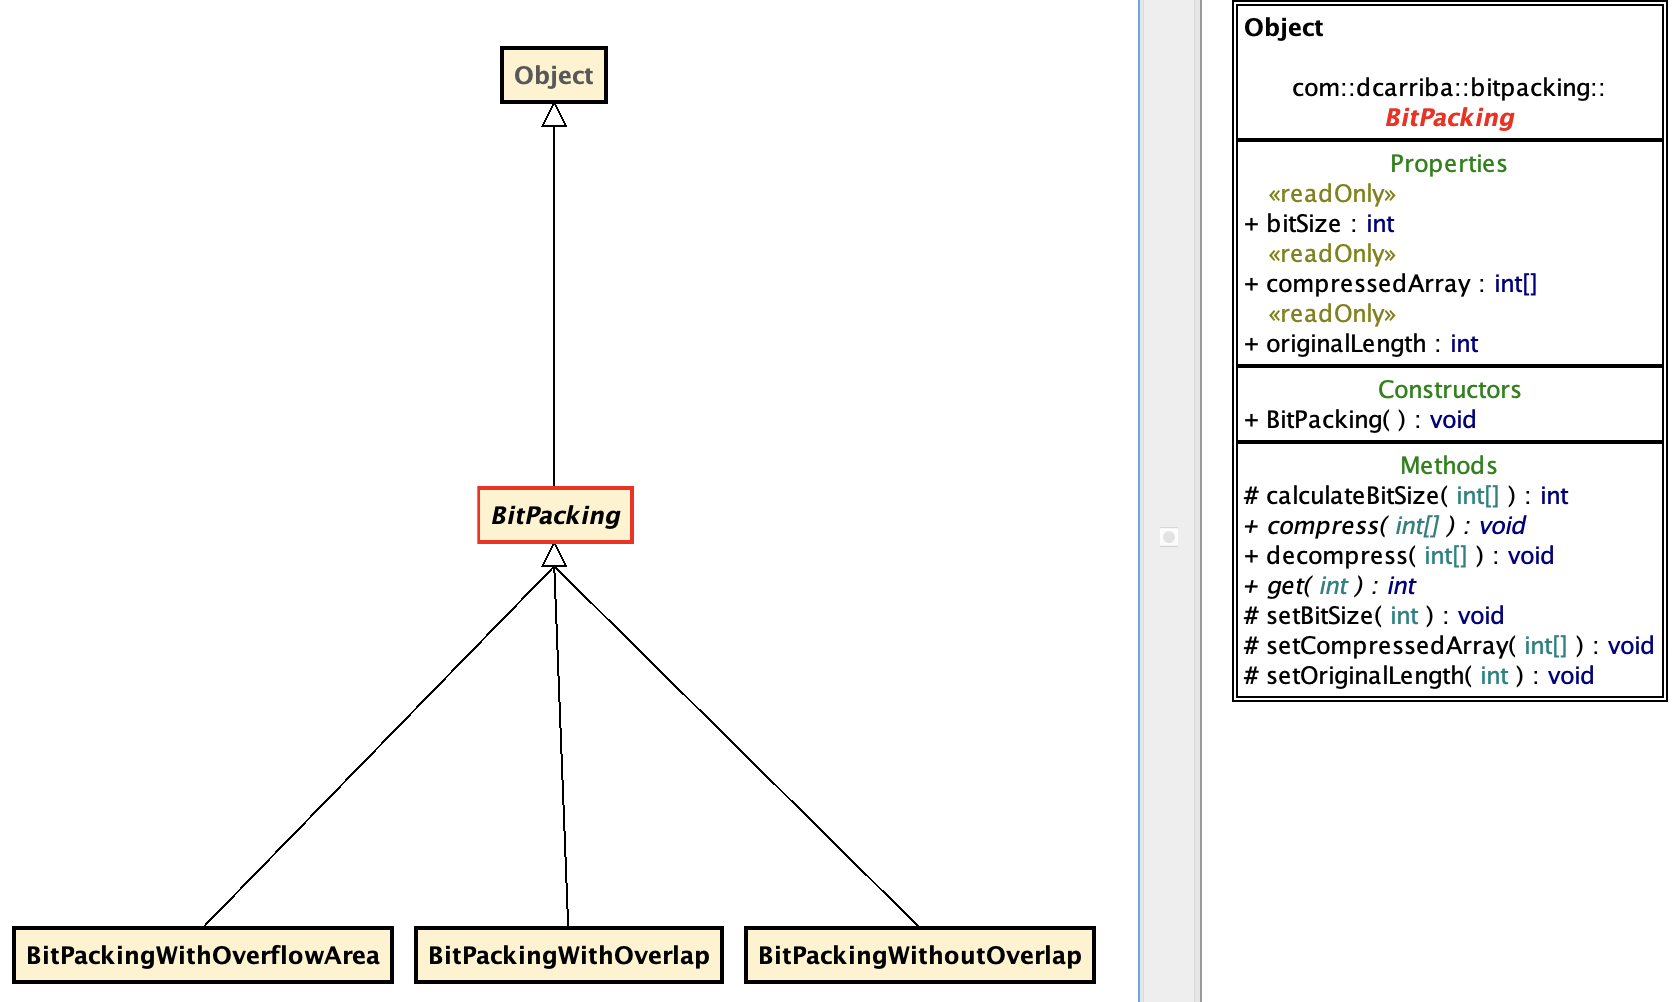
\includegraphics[width=0.8\textwidth]{img/BitPackingUML.png}
    \caption{Schéma UML \textsl{BitPacking}}
    \label{fig:BitPackingUML}
\end{figure}



\subsubsection{Implémentation commune à toutes les versions}

Toutes les versions de "Bit Packing" héritent donc d'une classe abstraite \textsl{BitPacking}. Celle-ci contient les champs (i.e. les attributs) ainsi que les méthodes communes à toutes les versions différentes, soit :
\begin{itemize}
\item le contenu du tableau compressé
\item la taille du tableau original
\item le nombre de bits sur lequel chaque valeurs sera codé dans le tableau compressé
\item une méthode pour calculer ce nombre de bits
\item une méthode de décompression commune, qui récupère chaque élément d'index i grâce à la méthode :
\begin{lstlisting}[language=Java] 
public abstract int get(int i); 
\end{lstlisting} 
(implémenté dans chaque version)
\end{itemize}
\par Une classe \textsl{BitPackingTest} a également été implémenté contenant des tests unitaires pour tester le bon fonctionnement de la méthode calculant le nombre de bits sur lequel chaque valeurs sera codé dans le tableau.



\subsection{Bit Packing with overlap}

La première version de "Bit Packing" de ce projet est une version nommé "with overlap". Cela signifie que une valeur, du tableau à compresser, peut être compressé sur deux entiers consécutifs au sein du tableau compressé.


\subsubsection{Implémentation}

Cette version de "Bit Packing" a été implémenté par la classe \textsl{BitPackingWithOverlap} qui hérite de la classe abstraite \textsl{BitPacking}.
\par \textsl{BitPackingWithOverlap} implémente les méthodes abstraites de \textsl{BitPacking}, soit :
\begin{lstlisting}[language=Java]
@Override
public void compress(int[] array) {
	...
}
@Override
public int get(int i) {
	...
}
\end{lstlisting}
\par Une classe \textsl{BitPackingWithOverlapTest} a également été implémenté contenant des tests unitaires pour tester le bon fonctionnement de la compression, décompression et accès au i-ème élément.


\subsubsection{Fonctionnement}

\paragraph{Compression :} la compression fonctionne de la manière suivante :
\begin{itemize}
\item on calcule le nombre de bits nécessaire pour coder la plus grande valeur du tableau initial, afin de codé toutes les valeurs sur ce nombre de bits
\item on donc calculer le nombre d'entiers de 32 bits nécessaire pour contenir toutes les valeurs compressé, ce qui est donc la taille du tableau compressé
\item pour chaque valeur du tableau inital, on le code sur le premier entier où il peut être compressé, et si il ne peut pas être contenu entièrement sur cet entier, on continue de le compresser sur l'entier suivant.
\end{itemize}
\par Ainsi chaque valeur du tableau initial est codé sur N bits (i.e. le nombre de bits nécessaire pour coder la plus grande valeur du tableau initial) sur un entier du tableau compressé, ou sur deux entiers consécutifs du tableau compressé si il ne peut être contenu entièrement sur le premier entier.

\paragraph{Accès au i-ème élément :} l'accès au i-ème élément fonctionne de la manière suivante :
\begin{itemize}
\item on connait le nombre de bits sur lequel toutes les valeurs ont été codées, donc il suffit de calculer sur quel entier de 32 bits la i-ème valeur à été compressé. 
\item on calcul la position de la i-ème valeur au sein de cet entier (de 32 bits), et on extrait la valeur, puis la renvoie. Si la i-ème valeur n'est pas entièrement compressé sur cet entier, on continu de l'extraire l'entier suivant .
\end{itemize}


\paragraph{Décompression :} la décompression fonctionne de la manière suivante :
\begin{itemize}
\item pour tout valeur i il suffit d'utiliser la méthode pour accéder au i-ème élément pour la récupérer 
\item toutes les valeurs récupérés peuvent ainsi être rétablis dans le tableau décompressé
\end{itemize}



\subsection{Bit Packing without overlap}

La seconde version de "Bit Packing" de ce projet est une version nommé "without overlap". Cela signifie que une valeur, du tableau à compresser, sera toujours compressé sur un seul, et non deux, entier du tableau compressé.


\subsubsection{Implémentation}

Cette version de "Bit Packing" a été implémenté par la classe \textsl{BitPackingWithoutOverlap} qui hérite de la classe abstraite \textsl{BitPacking}.
\par \textsl{BitPackingWithoutOverlap} implémente les méthodes abstraites de \textsl{BitPacking}, soit :
\begin{lstlisting}[language=Java]
@Override
public void compress(int[] array) {
	...
}
@Override
public int get(int i) {
	...
}
\end{lstlisting}
\par Une classe \textsl{BitPackingWithoutOverlapTest} a également été implémenté contenant des tests unitaires pour tester le bon fonctionnement de la compression, décompression et accès au i-ème élément.


\subsubsection{Fonctionnement}

\paragraph{Compression :} la compression fonctionne de la manière suivante :
\begin{itemize}
\item on calcule le nombre de bits nécessaire pour coder la plus grande valeur du tableau initial, afin de codé toutes les valeurs sur ce nombre de bits
\item on calcule ensuite le nombre de valeurs qui peuvent être codés sur un seul entier de 32 bits, et par conséquent la taille du tableau compressé
\item pour chaque valeur du tableau inital, on le code sur le premier entier où il peut être contenu entièrement
\end{itemize}
\par Ainsi chaque valeur du tableau initial est codé sur N bits (i.e. le nombre de bits nécessaire pour coder la plus grande valeur du tableau initial) d'un entier (32 bits) du tableau compressé.

\paragraph{Accès au i-ème élément :} l'accès au i-ème élément fonctionne de la manière suivante :
\begin{itemize}
\item on connait le nombre de bits sur lequel toutes les valeurs ont été codées, donc il suffit de calculer sur quel entier de 32 bits la i-ème valeur est situé. 
\item on calcul la position de la i-ème valeur au sein de cet entier (de 32 bits), et on extrait la valeur, puis la renvoie.
\end{itemize}


\paragraph{Décompression :} la décompression fonctionne de la manière suivante :
\begin{itemize}
\item pour tout valeur i il suffit d'utiliser la méthode pour accéder au i-ème élément pour la récupérer 
\item toutes les valeurs récupérés peuvent ainsi être rétablis dans le tableau décompressé
\end{itemize}


\subsection{Bit Packing with overflow areas}

La troisième version de "Bit Packing" de ce projet est une version nommé "with overflow areas". Elle fonctionne de la manière suivante :
\par Si un nombre du tableau initial nécessite un grand nombre de bits k et que les autres nombres nécessitent seulement k' bits avec k' < k, il est inutile de représenter tous les nombres avec k bits. Dans ce cas, nous pouvons attribuer une valeur spéciale à un entier compressé pour indiquer que sa valeur réelle se trouve ailleurs, à une position spécifique du tableau, appelée zone de débordement, ou "overflow area".
\par Par exemple, si nous voulons encoder les nombres 1, 2, 3, 1024, 4, 5 et 2048, nous pouvons encoder 1, 2, 3 et 4 sur 3 bits et les autres nombres sur 11 bits.
\par Nous utiliserons un bit du codage pour indiquer que nous ne représentons pas directement un nombre, mais une position dans la zone de débordement. Si 1 correspond à la zone de débordement, et si x-y signifie que le premier bit vaut x et les suivants y, nous représenterons la séquence de nombres 1, 2, 3, 1024, 4, 5, 2048 par : 0-1, 0-2, 0-3, 1-0, 0-4, 0-5, 1-1, 1024, 2048.

\subsubsection{Implémentation}

Cette version de "Bit Packing" a été implémenté par la classe \textsl{BitPackingWithOverflowArea} qui hérite de la classe abstraite \textsl{BitPacking}.
\par \textsl{BitPackingWithOverflowArea} implémente les méthodes abstraites de \textsl{BitPacking}, soit :
\begin{lstlisting}[language=Java]
@Override
public void compress(int[] array) {
	...
}
@Override
public int get(int i) {
	...
}
\end{lstlisting}
Ainsi que une méthode de décompression plus efficace pour \textsl{BitPackingWithOverflowArea} que celle déjà existante de \textsl{BitPacking} :
\begin{lstlisting}[language=Java]
@Override
public void decompress(int[] array) {
	...
}
\end{lstlisting}

\par Une classe \textsl{BitPackingWithOverflowAreaTest} a également été implémenté contenant des tests unitaires pour tester le bon fonctionnement de la compression, décompression et accès au i-ème élément.


\subsubsection{Fonctionnement}

\paragraph{Compression :} la compression fonctionne de la manière suivante :
\begin{itemize}
\item on calcule N le nombre de bits nécessaire pour coder la plus grande valeur du tableau initial. Toute valeur qui doit réellement être codé sur N bits sera une valeur compressé dans la "overflow area", et les autres valeurs, qui peuvent être codés sur N' < N bits, seront compressé sur N' bits de manière normale.
\item pour toutes les valeurs du tableau initial, on compresse dont soit la valeur sur N' bit (en ajoutant un bit 0 supplémentaire avant), soit on compresse l'index de la valeur dans l' "overflow area" (en ajoutant un bit 1 supplémentaire avant). A la fin, toutes les valeurs de l' "overflow area", i.e. les valeurs compressé sur N bits, seront ajoutés à la fin du tableau compressé.
\end{itemize}
\par Ainsi les grandes valeurs (i.e. celles qui doivent être compressé sur N bits) seront compressé dans l' "overflow area", à la fin du tableau compressé, et avant dans le tableau compressé sera seulement une référence (de forme 1-overflowValueIndex) à sa position au sein de l' "overflow area".

\paragraph{Décompression :} la décompression fonctionne de la manière suivante :
\begin{itemize}
\item on parcours le tableau compressé de bit en bit.
\item Si le bit indicateur est 0 alors cela signifie que la valeur a été compressé de manière normale sur N' bits. On peut donc facilement la décompresser et ajouter au tableau de résultat.
\item Si le bit indicateur est 1 alors cela signifie que la valeur a été compressé dans l' "overflow area". On sauvegarde donc l'indice actuel où la valeur devrait être, pour compléter l'indice à la fin lors de la décompression de la valeur de l' "overflow area"
\end{itemize}

\paragraph{Accès au i-ème élément :} l'accès au i-ème élément fonctionne de la manière suivante :
\begin{itemize}
\item pour pouvoir déterminer si la i-ème valeur a été compressé de manière normale sur N' bits, ou dans l' "overflow area" sur N bits, il est nécessaire de parcourir le tableau compressé de bit en bit pour lire les bits indicateurs (0, ou 1 si la valeur est compressé dans l' "overflow area"). Ce procédé revient exactement à faire une décompression, comme l'entièreté du tableau compressé, pour notamment extraire les valeurs des éléments compressé dans l' "overflow area".
\item ainsi on décompresse temporairement le tableau pour pouvoir donné la valeur du i-ème élément.
\end{itemize}


\clearpage




\section{Tests Unitaires}

\subsection{Implémentation}

Pour vérifier le bon fonctionnement des méthodes pour compresser, décompresser at accéder au i-ème élément du tableau compressé, on a implémenter des tests unitaires pour les classes de "Bit Packing". Ces tests unitaires sont situés dans le répertoire :
\begin{lstlisting}
./src/test/java/
\end{lstlisting}
\par Les tests unitaires implémentés sont :
\begin{itemize}
\item \textsl{BitPackingTest} contient les tests unitaires pour \textsl{BitPacking}
\item \textsl{BitPackingWithOverlapTest} contient les tests unitaires pour \textsl{BitPackingWithOverlap}
\item \textsl{BitPackingWithoutOverlapTest} contient les tests unitaires pour \textsl{BitPackingWithoutOverlap}
\item \textsl{BitPackingWithOverflowAreaTest} contient les tests unitaires pour \textsl{BitPackingWithOverflowArea}
\end{itemize}
\par \textsl{BitPackingWithOverlapTest}, \textsl{BitPackingWithoutOverlapTest} et \textsl{BitPackingWithOverflowAreaTest} étendent la classe \textsl{BitPackingVersionsBaseTest} qui contient la logique des tests unitaire, commune pour ces 3 versions de "Bit Packing".

\subsection{Visualisation des résultats des tests}

Les tests unitaires sont exécutés avec la commande suivante :
\begin{lstlisting}[language=Bash]
./gradlew test
\end{lstlisting}
Si "BUILD SUCCESSFUL" s'affiche, alors tout les tests unitaires on été exécutés avec succès.
\par Une visualisation sur l'ensemble des résultats est également disponible sur :
\begin{lstlisting}[language=Bash]
./build/reports/tests/test/index.html
\end{lstlisting}
\begin{figure}[h!]
    \centering
    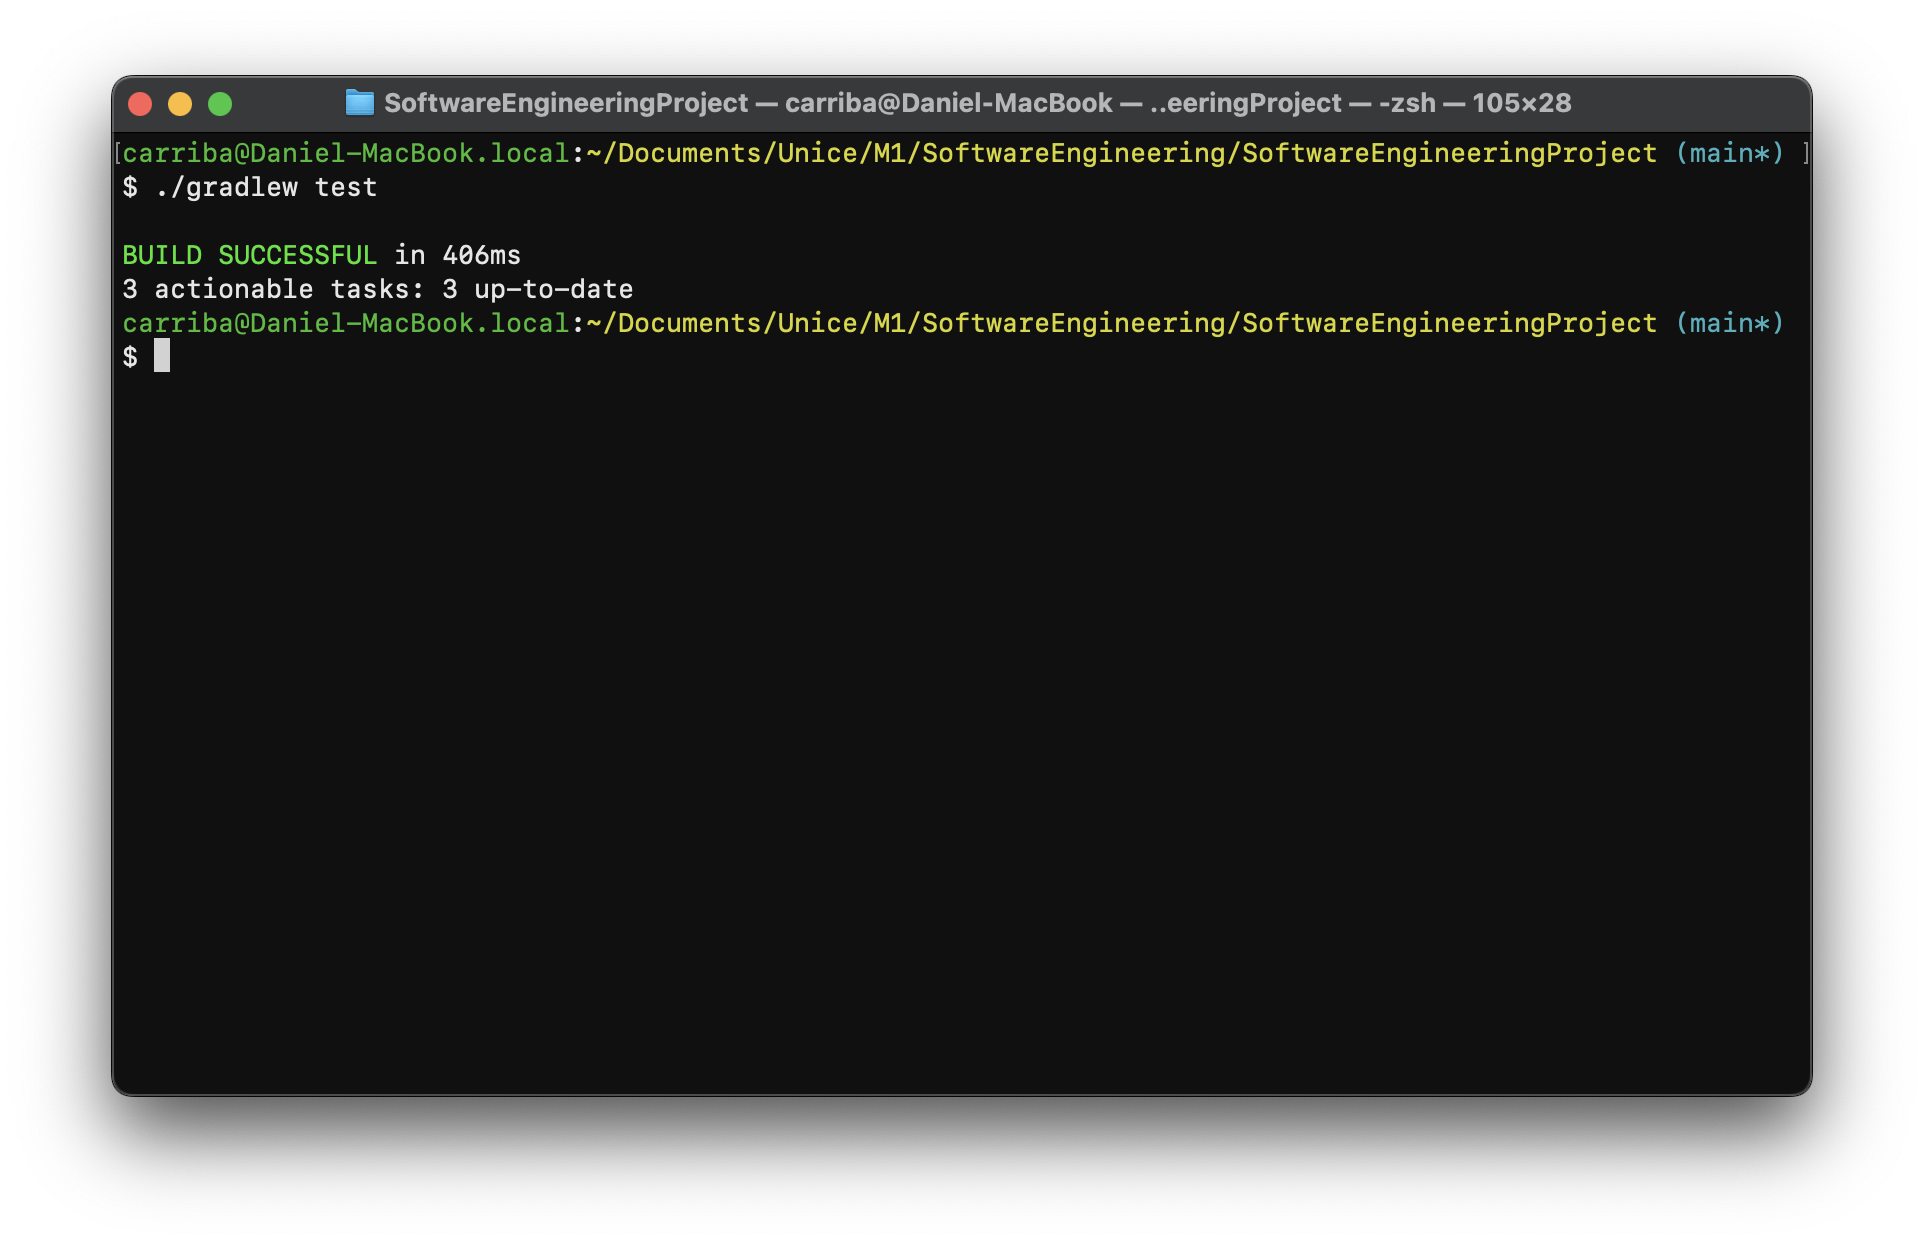
\includegraphics[width=1\textwidth]{img/unitTestsTerminal.png}
    \caption{Tests unitaires exécutés avec succès}
    \label{fig:unitTestsTerminal}
\end{figure}
\begin{figure}[h!]
    \centering
    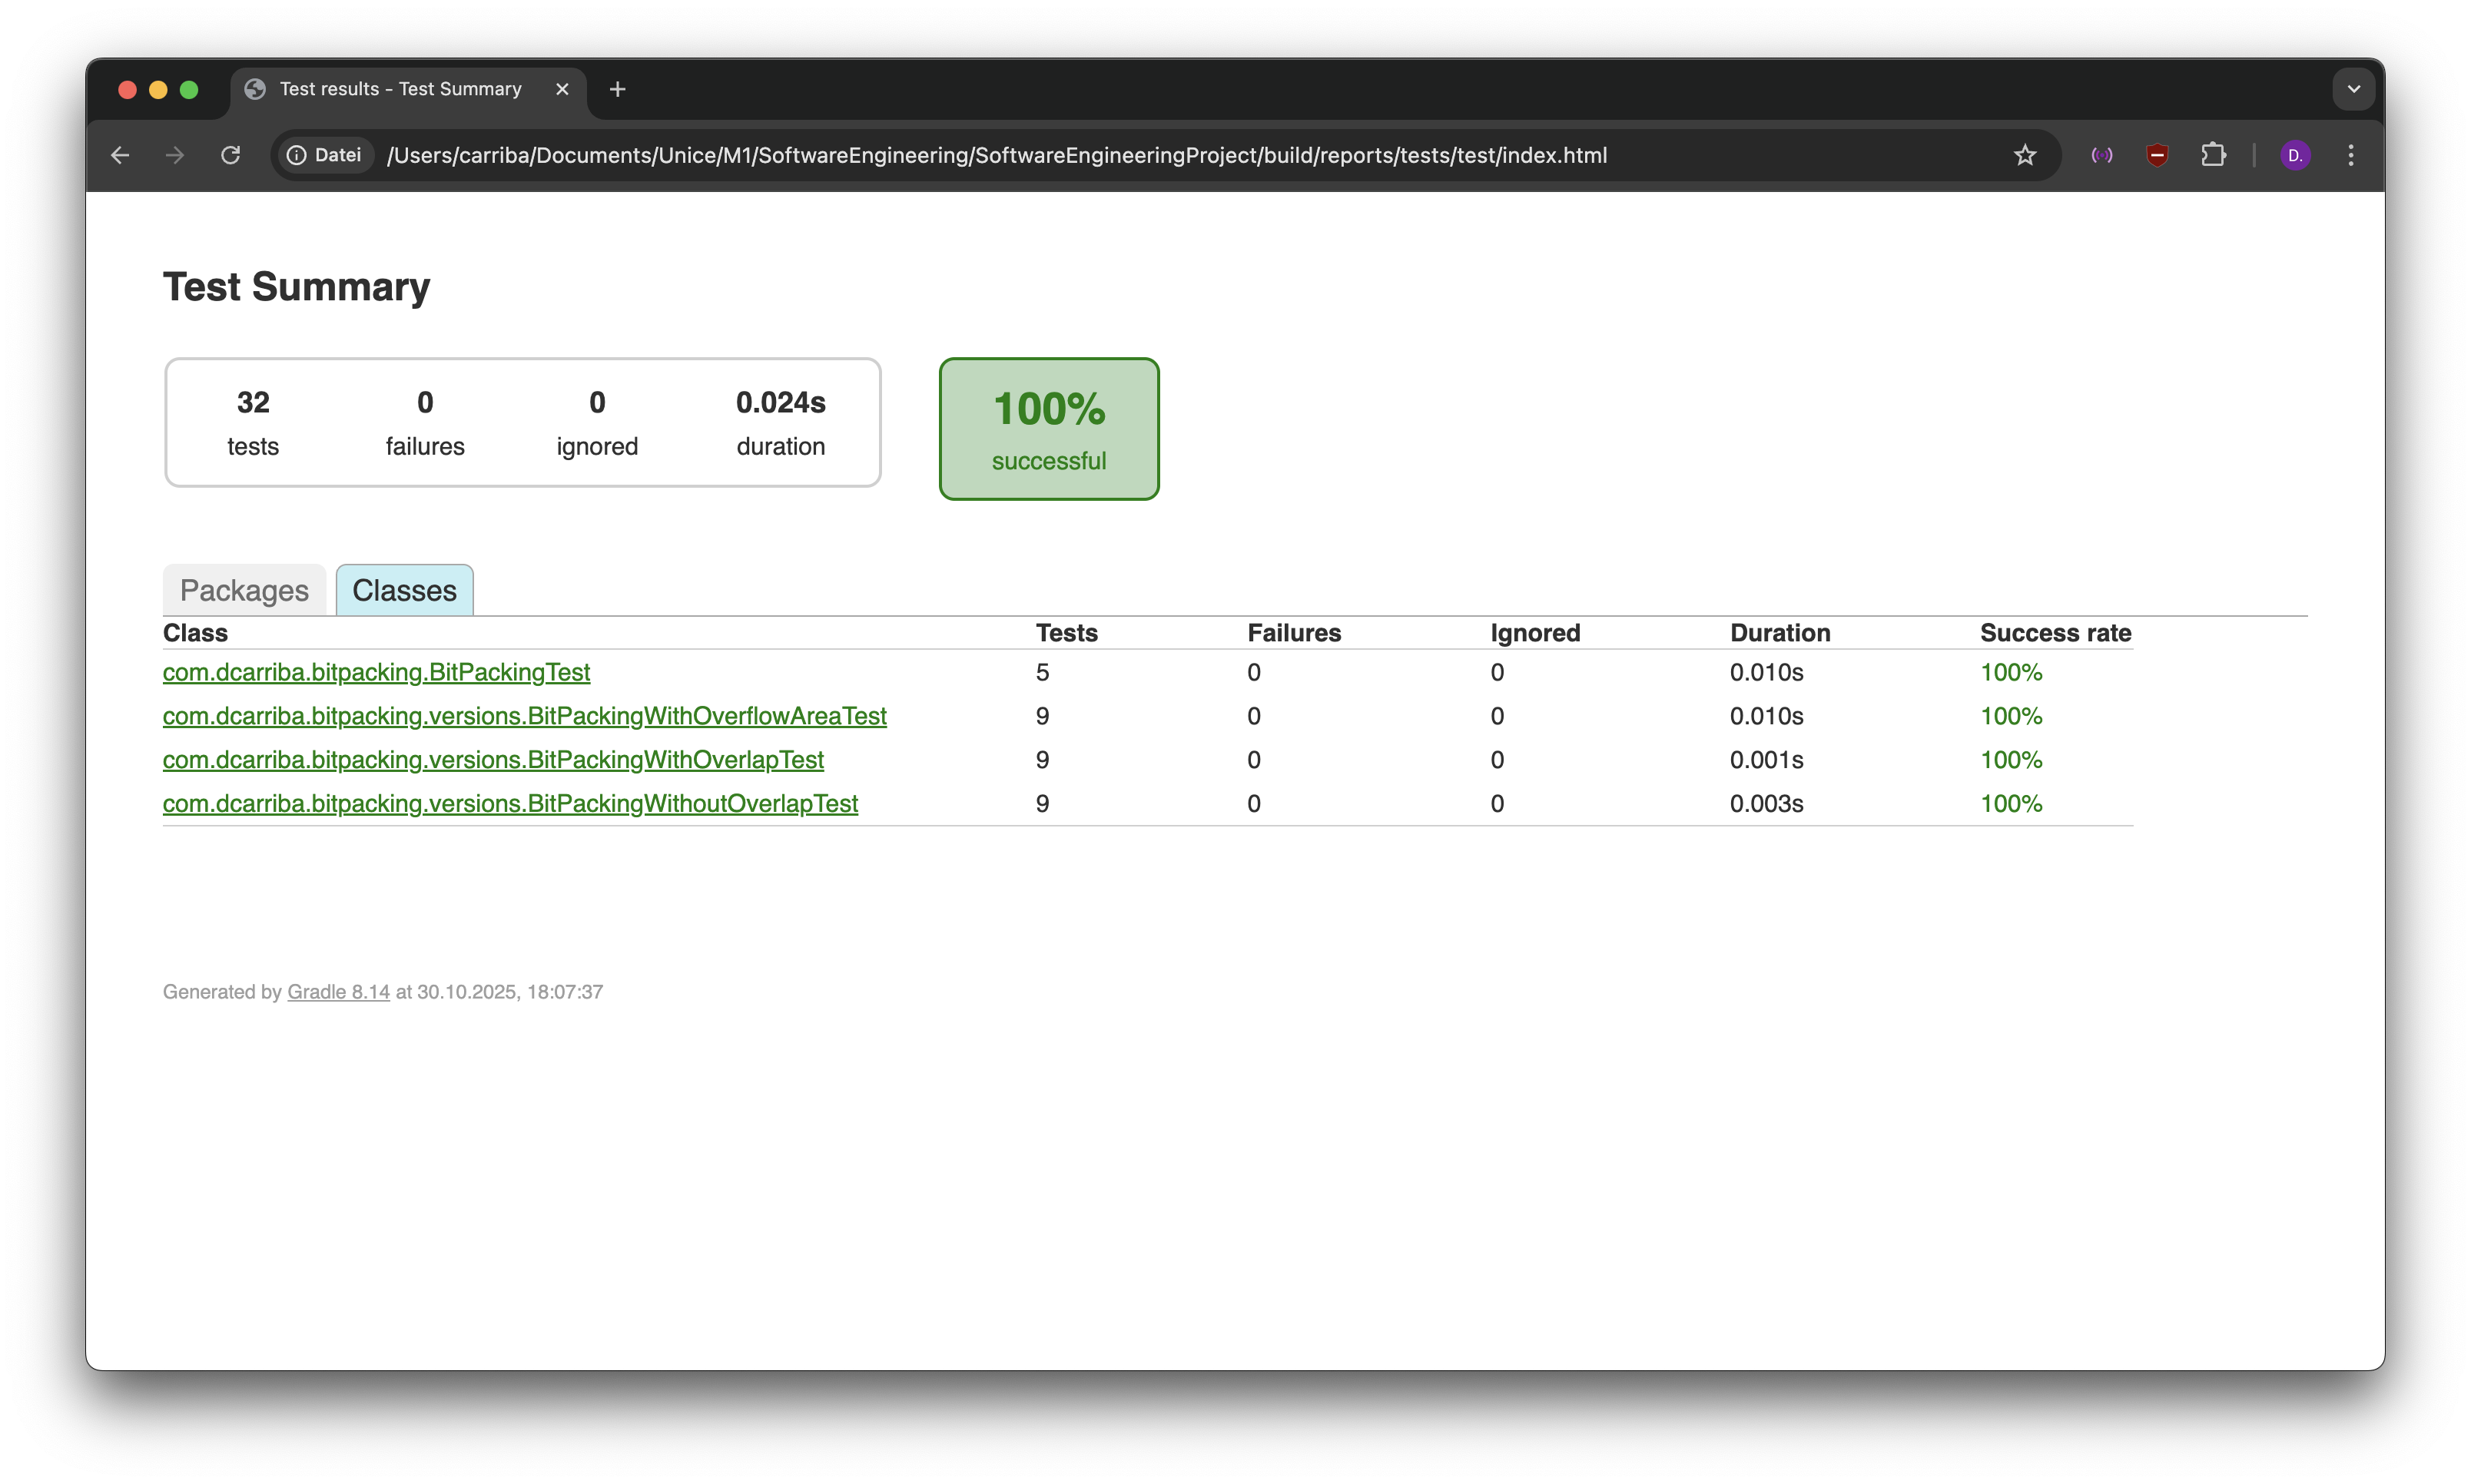
\includegraphics[width=1\textwidth]{img/unitTestsResults.png}
    \caption{Visualisation des résultats des tests unitaires}
    \label{fig:unitTestsResults}
\end{figure}



\clearpage




\section{Benchmarks}

\subsection{Protocole pour mesurer le temps}

Pour mesurer la performance en temps des méthodes des différentes versions de "Bit Packing", on a choisit un protocole constitué des étapes suivantes.

\subsubsection{Phase "warm-up"}

Avant de mesurer les temps, il est important de faire une phase de "warm-up" (échauffement), afin d'assurer que les optimisations de la JVM, comme la compilation "Just-in-time", n'affecte pas les résultats finaux du benchmark.

\subsubsection{Mesures des temps}

La mesure de temps s'effectue grâce à la "Java Virtual Machine's high-resolution time source" en nano-secondes :
\begin{lstlisting}[language=Java] 
System.nanoTime(); 
\end{lstlisting} 
qui est appelé avant et après l'execution de la méthode à mesurer. La différence entre ces 2 temps nous donne donc le temps écoulé pendant l'exécution de la méthode à mesurer.
\par La classe \textsl{TimeBenchmarks} implémente les méthodes pour mesurer ainsi le temps pour les méthodes de compression, décompression et accès au i-ème élément du tableau compressé.

\subsubsection{Calcul du temps moyen sur des entrées variables}

Nous choisissons de prendre la moyenne sur un nombre N (ici 10, mais modifiable grâce à une constante dédiée dans la classe \textsl{Config}) de répétitions de mesures de temps. De plus, à chaque répétition le tableau obtient de nouvelles valeurs aléatoires. Ceci nous assure donc un calcul de temps moyens plus fiable.
\par Ces benchmarks sont exécutés à plusieurs reprises avec plusieurs tableaux de taille différents, pour ainsi obtenir des temps moyens pour des tailles de tableaux différents, et donc pouvoir comparer les temps par rapport à la version de \textsl{BitPacking} et par rapport à la taille du tableau en entrée.
\par La classe \textsl{RunTimeBenchmarks} s'occupe d'exécuter ces benchmarks, et est appelée dans la fonction main de la classe \textsl{Main}.


\subsection{Protocole pour mesurer le taux de compression}

\subsubsection{Mesures des taux de compression}

La mesure du taux de compression s'effectue en compressant un tableau, et en calculant le résultat  de la division suivante :
\begin{lstlisting}[language=Java] 
bitPacking.getCompressedArray().length / array.length
\end{lstlisting} 
où "bitPacking" est un objet de type \textsl{BitPacking} qui contient le tableau compressé de "array"
\par La classe \textsl{CompressionRatioBenchmarks} implémente la méthodes qui effectue ce calcul de taux de compression

\subsubsection{Calcul du taux moyen sur des entrées variables}

Nous choisissons de prendre la moyenne sur un nombre N (ici 10, mais modifiable grâce à une constante dédiée dans la classe \textsl{Config}) de répétitions de mesures de taux de compression. De plus, à chaque répétition le tableau obtient de nouvelles valeurs aléatoires. Ceci nous assure donc un calcul du taux de compression plus fiable.
\par Ces benchmarks sont exécutés à plusieurs reprises avec plusieurs tableaux contenant chacun des valeurs maximales différentes. Ainsi on peut donc comparer le taux de compression des différentes versions en fonction des valeurs contenus à l'intérieur des tableaux en entrée.

\subsection{Exemple de résultats des benchmarks}

{\lstset{basicstyle=\scriptsize\ttfamily}
\begin{lstlisting} 
$ ./gradlew run                

> Task :run
__________________________________
| *** BIT PACKING BENCHMARKS *** |
__________________________________

*** Compression Ratio Benchmarks ***

Results of the compression ratio benchmarks, using randomly generated arrays
with different possible maximum values:

=== Average Compression Ratio (average over 10 repetitions) ===
Max Possible Value      With Overlap       Without Overlap    With Overflow Area
1                       0,03               0,03               0,38              
10                      0,13               0,13               0,18              
100                     0,22               0,25               0,33              
256                     0,25               0,25               0,41              
1000                    0,31               0,33               0,46              
5000                    0,41               0,50               0,46              
10000                   0,44               0,50               0,49              
2097151                 0,66               1,00               0,82              
16777215                0,75               1,00               0,91              
1073741823              0,94               1,00               1,09              
2147483647              0,97               1,00               1,13              

______________________________

*** Time Benchmarks ***

Warming up the JVM for better results...
Warm-up completed.

Results of the time measurements benchmarks, using randomly generated arrays
at different sizes:

=== Average Compression Time (in micro-seconds) (average over 10 repetitions) ===
Array Size   With Overlap       Without Overlap    With Overflow Area
100          0,82               0,31               7,15              
500          3,59               0,86               95,45             
1000         7,02               1,68               331,11            
5000         33,59              7,84               7566,23           

=== Average Decompression Time (in micro-seconds) (average over 10 repetitions) ===
Array Size   With Overlap       Without Overlap    With Overflow Area
100          3,85               2,39               1,89              
500          8,08               7,19               8,57              
1000         5,96               8,40               16,58             
5000         21,68              7,68               86,25             

=== Average Get Time (in nano-seconds) (average over 10 repetitions) ===
Array Size   With Overlap       Without Overlap    With Overflow Area
100          5,50               2,20               1167,80           
500          5,00               2,00               6083,40           
1000         5,10               2,40               12364,90          
5000         5,00               2,00               70411,00          

BUILD SUCCESSFUL in 8s
2 actionable tasks: 1 executed, 1 up-to-date
\end{lstlisting}
}

\subsection{Interprétation des benchmarks obtenus}

\subsubsection{Benchmarks de taux de compression}

On peut remarquer que la version "With Overlap" a un taux de compression toujours meilleurs que les autres versions de la méthode de compression.
\par De plus on remarque que les taux de compression de chaque version est différent de la valeur maximale contenu dans le tableau à compressé. Ainsi plus cette valeur maximale est inférieur, mieux le taux de compression est.
\par Le taux de compression de la version "Without Overlap" est le second meilleur si la valeur maximale du tableau à compressé est particulièrement petite ou grande. Sinon pour une valeur maximale relativement moyenne, la version "With Overflow Area" donne de meilleurs taux que la version "Without Overlap". Pour des petites valeurs maximales, la version "With Overflow Area" n'est pas très optimisé, et pour des valeurs maximales très élevées, la version "With Overflow Area" a même un tableau compressé de taille plus grande que le tableau original.
\par Ainsi on peut donc conclure que la version "With Overlap" donne toujours le meilleurs taux de compression, et que la version "With Overflow Area" n'est pas adapté si la valeur maximale du tableau à compressé est particulièrement petite ou particulièrement grande. 


\subsubsection{Benchmarks de temps}

On peut remarquer que la version "Without Overlap" à presque toujours les meilleurs temps pour la compression, la décompression et pour l'accès au i-ème élément du tableau compressé.
\par La version "With Overlap" a également des temps correctes vis-à-vis de la compression, décompression et accès au i-ème élément.
\par Cependant, la version "With Overflow Area" a dans la majorité des cas les temps les plus élevées. Notamment pour l'accès au i-ème élément on remarque un temps particulièrement élevée. Ceci-ci est surement dû à mon implémentation de cette méthode, qui est obligée de systématiquement décompresser le tableau avant de pouvoir déterminer le i-ème élément. 
\par Ainsi on peut donc conclure que les meilleurs versions de "Bit Packing" en fonction du temps sont les versions "Without Overlap" suivi par "With Overlap" et finalement "With Overflow Area", qui a des temps considérablement supérieur au autres versions. 

\subsubsection{Conclusion sur les benchmarks}

Grâce au différents benchmarks obtenus, on peut conclure que la meilleur version de "Bit Packing" en considérant le temps de compression, décompression et accès au i-ème est la version "Without Overlap".
\par Si on considère le taux de compression, on peut conclure que la version "With Overlap" de "Bit Packing" offre les meilleurs résultats. 

\clearpage



\section{Temps de transmission pour une latence t où la compression devient utile}

Pour déterminer si, et quand, la compression de tableaux d'entiers positifs est utile pour répondre au problème initiale, soit la transmission de ces tableau à travers internet, ce projet calcule le temps de transmission pour une latence t où la compression devient utile, pour chaque version de la compression "Bit Packing" qui a été implémenté.

\subsection{Protocole pour le calcul}

Le calcul est effectué par la classe \textsl{CalculateTransmissionTimeAndIfWorth}, qui calcule :
\begin{itemize}
\item le temps de transmission du tableau sans compression
\item pour chaque version de compression : le temps de transmission du tableau compressé (à l'aide du temps de compression et de décompression, calculé par les benchmarks de temps)
\item si la compression est utile, i.e. si le temps de transmission du tableau compressé (qui inclus le temps de compression et de decompression) est inférieur au temps de transmission du tableau non compressé
\end{itemize}
Pour les calculs de transmission, on a choisi d'assumer pour le taux de transmission la moyenne, qui est de 10 Mbps.

\subsection{Calcul sur des entrées variables}

La classe \textsl{RunCalculateTransmissionTimeAndIfWorth} utilise donc la classe présentés précédemment pour effectuer les calculs sur des tableaux en entrées avec des tailles différentes, et avec des éléments de valeurs maximales possibles différentes également, pour des résultats sur des entrées un maximum variées.

\subsection{Exemple de résultats}

{\lstset{basicstyle=\scriptsize\ttfamily}
\begin{lstlisting}
$ ./gradlew run

> Task :run
__________________________________
| *** BIT PACKING BENCHMARKS *** |
__________________________________

***     Transmission Time calculation      ***
*** and if the compression is worth or not ***

=== Using an array with size 1000 ===
Max Possible Value   T_without    With Overlap          Without Overlap       With Overflow Area   
                                  T_time     is worth?  T_time     is worth?  T_time     is worth? 
1                    0,003200     0,000376   true       0,000252   true       0,001955   true      
10                   0,003200     0,000502   true       0,000465   true       0,002286   true      
100                  0,003200     0,000816   true       0,000855   true       0,001437   true      
256                  0,003200     0,000892   true       0,000853   true       0,001746   true      
1000                 0,003200     0,001105   true       0,001121   true       0,001899   true      
5000                 0,003200     0,001358   true       0,001656   true       0,001855   true      
10000                0,003200     0,001433   true       0,001656   true       0,001937   true      
2097151              0,003200     0,002136   true       0,003257   false      0,003048   true      
16777215             0,003200     0,002431   true       0,003255   false      0,003387   false     
1073741823           0,003200     0,003051   true       0,003257   false      0,003949   false     
2147483647           0,003200     0,003136   true       0,003256   false      0,004070   false     

=== Using an array with size 15000 ===
Max Possible Value   T_without    With Overlap          Without Overlap       With Overflow Area   
                                  T_time     is worth?  T_time     is worth?  T_time     is worth? 
1                    0,048000     0,001890   true       0,001892   true       0,025311   true      
10                   0,048000     0,006191   true       0,006166   true       0,028015   true      
100                  0,048000     0,010658   true       0,012223   true       0,044309   true      
256                  0,048000     0,012107   true       0,012074   true       0,051079   false     
1000                 0,048000     0,015129   true       0,016064   true       0,065315   false     
5000                 0,048000     0,019623   true       0,024045   true       0,061644   false     
10000                0,048000     0,021127   true       0,024045   true       0,072288   false     
2097151              0,048000     0,031640   true       0,048048   false      0,117700   false     
16777215             0,048000     0,036134   true       0,048046   false      0,122586   false     
1073741823           0,048000     0,045163   true       0,048051   false      0,131956   false     
2147483647           0,048000     0,046672   true       0,048055   false      0,134984   false     

Notice:
- "T_without" is the Transmission Time (in seconds) of the array without compression
- for each compression version "T_time" is the Transmission Time (in seconds) of the array,
compressed using that compression version
- for each compression version "is worth?" indicates if the compression was worth,
i.e. if it improved the Transmission Time
- in the calculations the average transmission rate of 10 Mbps is used

BUILD SUCCESSFUL in 3s
2 actionable tasks: 2 executed
\end{lstlisting}
}

\subsection{Interprétation des résultats obtenus}

Les résultats obtenus ci-dessus montrent pour les tableaux des taille 1000 et 15000, pour chaque valeur maximale possible, le temps de transmission du tableau non compressé (représenté par la colonne "T without"), ainsi que pour chaque version de compression "Bit Packing" le temps de transmission du tableau compressé (représenté par la colonne "T time"). Si "T time" est inférieur à "T without", alors la compression s'est avéré utile et bénéfique pour améliorer le temps de transmission. Ceci est représenté par la colonne "is worth?".
\par Ainsi on remarque donc que la version de compression "With Overlap" améliore toujours le temps de transmission du tableau.
\par La version de compression "Without Overlap" améliore le temps de transmission du tableau seulement si la valeur maximal possible dans le tableau ne dépasse un certain seuil (entre 10000 et 2097151 d'après nos résultats).
\par La version de compression "With Overflow Area" améliore le temps de transmission seulement si la valeur maximal possible du tableau est en dessous d'un seuil. Ce seuil dépend, comme on peut le remarquer, de la taille du tableau en entier. Si la taille du tableau est de 1000 alors la version de compression "With Overflow Area" est utile seulement si la valeur maximale possible est inférieur 2097151, alors que si la taille du tableau est de 15000, "With Overflow Area" est seulement utile si la valeur maximale possible est de 100.
\par Les versions "With Overlap" et "Without Overlap" ne dépendent pas de la taille du tableau, mais seulement de la valeur maximale possible au sein du tableau, au contraire de la version de compression "With Overflow Area".

\subsection{Conclusion sur les temps de transmissions}

Grâce à nos résultats obtenus, on peut donc conclure que la version "With Overlap", de la méthode de compression de "Bit Packing", améliore toujours le temps de transmission d'un tableau d'entiers positifs par internet, comparé au temps de transmission de ce tableau sans le compressé. Au contraire, les versions "Without Overlap" et "With Overflow Area" n'améliorent pas toujours ce temps de compression. Ainsi compresser le tableau avec la version "With Overlap" de "Bit Packing" s'avère utile et bénéfique pour améliorer le temps de transmission de tableau d'entiers positifs par internet.

\clearpage


\section{Tableaux avec des nombres négatifs}

Considérons que les tableaux à transmettre peuvent contenir des nombres négatifs. Nous expliquerons le problème que ceci pourrait causer avec la méthode de compression "Bit Packing" implémenté par ce projet. Nous proposerons également une solution possible, pour résoudre ce problème.

\subsection{Problème}

Comparé à des nombres positifs, le codage binaire de nombres négatifs est différent. En effet, il s'effectue grâce au complément à deux. Ainsi les nombres négatifs on pour caractéristique que le bit de poids fort est un "1", et que l'ensemble du codage binaire est en complément à deux.
\par La méthode de compression "Bit Packing" compresse les nombres en supprimants tout les bits "0" inutiles au codage binaire du nombre à compressé. Comme les nombres négatifs sont codés en complément à deux, les "0" inutiles deviennent des "1", et ainsi il est impossible de compresser ces nombres négatifs avec l'implémentation actuelle de "Bit Packing".

\subsection{Solution possible}

Une solution possible pour remédier au problème décrit ci-dessus, serait d'utiliser le méthode d'encodage appelé "Zigzag encoding".
\par La méthode d'encodage "Zigzag encoding" est un encodage qui convertit en nombre positif les nombres négatifs. Il fait ceci en attribuant une nouvelle valeur positif pour chaque nombre, en alternant nombre positif et négatif.
\par Ainsi on aura par exemple : 0 devient 0, -1 devient 1, 1 devient 2, -2 devient 3, 2 devient 4, -3 devient 5, 3 devient 6, etc.
\par La méthode "Zigzag" peut donc facilement convertir les nombres négatifs en positifs, et peut également simplement reconstruire la valeur initiale, grâce à des formules mathématiques. Intégrer une méthode pour convertir tout les nombres en encodage "Zigzag" avant d'effectuer la compression avec notre méthode de "Bit Packing" serait donc une solution efficace pour résoudre le problème évoqué ci-dessus, et la méthode de compression "Bit Packing" pourrait donc fonctionner sur tout les nombres et non les nombres positifs seulement. 

\clearpage


\section{Conclusion}


\clearpage


\end{document}
